\documentclass{article}
\usepackage{graphicx,color}
\oddsidemargin=0in
\evensidemargin=0in
\topmargin=0in
\textheight=9in
\textwidth=6.5in
\headheight=0in
\headsep=0in
\makeatletter

\newcommand{\xsupp}{{\em xsupplicant}}

\begin{document}
\title{A Brief Architectural Overview to \xsupp}
\author{The Xsupp Guys}

\maketitle

\section{Introduction}
This document serves as an overview of the code structure of \xsupp.
It's intended purpose is to agree on a model to code to such that future
bug fixes, features, and other updates can be discussed in a more structured 
manner. This document, like \xsupp, is a work in progress.


\section{Current Code Flow}
The diagram below attempts to capture the current flow of information
through the \xsupp code. Note that this assumes normal
operation. Error conditions are outside the scope of this section,
unless explicitly stated. The following notation is used below:
  \begin{itemize}
    \item \textcolor{red}{File names} are in \textcolor{red}{red}.
    \item Function names are in black.
    \item \textcolor{blue}{Pseudocode} is in \textcolor{blue}{blue}.
    \item \textcolor{green}{Data} is in \textcolor{green}{green}.
  \end{itemize}
  

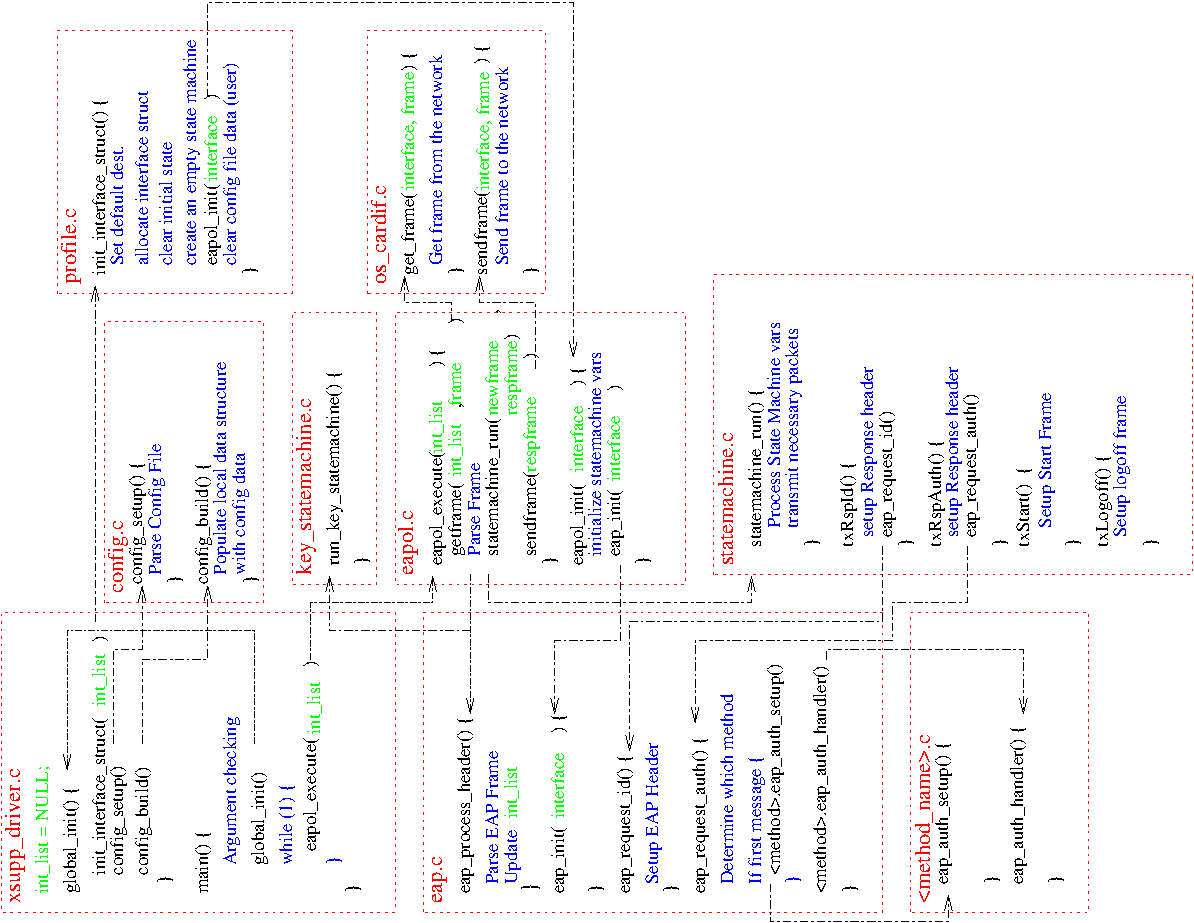
\includegraphics[angle=-90]{current_code_flow.pdf}

\section{Data Structures}
This section provides and overview to the various data structures used in 
xsupplicant. This is an overview, but is not guaranteed to be in sync
with the latest code. Do not rely on this document for coding, just for
an overview of how things are structured.

\end{document}
